\documentclass[60pt]{article}
\usepackage[a4paper, margin={1in, 1in}]{geometry}
\usepackage[utf8]{inputenc}
\usepackage{polski}
\usepackage{mathtools}
\usepackage{amsfonts}
\usepackage{amssymb}
\usepackage{amsmath}
\usepackage{multicol}
\usepackage{paralist}
\usepackage{tabto}
\usepackage{graphicx}
\usepackage{etoolbox}
\usepackage{changepage}
\usepackage{tasks}
\usepackage{pgfplots}
\usepackage{fancyhdr}
\usepackage{mathtools}
\usepackage{tikz}
\DeclarePairedDelimiter\ceil{\lceil}{\rceil}
\DeclarePairedDelimiter\floor{\lfloor}{\rfloor}
\usepackage{graphicx}

\usepackage{minted}
\usemintedstyle{autumn}

\DeclareMathOperator{\arctg}{arctg}
\DeclareMathOperator{\sh}{sh}
\DeclareMathOperator{\ch}{ch}
\DeclareMathOperator{\sgn}{sgn}

\let\arctan\relax
\DeclareMathOperator{\arctan}{arctg}
\let\tan\relax
\DeclareMathOperator{\tan}{tg}

\pagestyle{fancy}

%Ściana tekstu

%Ściana tekstu

\title{Projekt szkolnej bazy danych}
\author{Jakub Kołodziejczyk, Konrad Nowak, Wojciech Węgrzyn}


\begin{document}
\maketitle

\newpage
\tableofcontents

\newpage
\section{Wstęp}

\subsection{Cel projektu}

Nasza grupa obrała sobie za cel utworzenia bazy danych szkoły. Sugerowaliśmy się raczej działaniem szkół na poziomie licealnym, stąd też w naszej bazie danych pojawiają się koła naukowe, przedmioty fakultatywne czy stypendia. 

\subsection{Główne założenia}

Głównym założeniem naszej grupy było utworzenie bazy danych, która pozwalałaby organom zarządzającym na łatwą analizę dziejów szkolnych. 

Nasz projekt nie pretenduje do bycia zastępnikiem elektronicznego dziennika typu Librus czy Synerga. Staraliśmy się raczej stworzyć bazę, która będzie dawała przejrzyste informacje zarządzania organizacją szkoły, stąd też wprowadziliśmy specjalne tabele typu urlopy, dni wolne czy usprawiedliwienia. 

\subsection{Możliwości}

Wiele funkcji, procedur, wyzwalaczy i widoków w naszej bazie danych pozwalają na zautomatyzowane zarządzanie bazą danych szkoły od strony jej administracji. 

Potencjalny użytkownik naszego projektu z łatwością może błyskawicznie wyświetlić najbardziej potrzebne dane, takie jak średnia ocen wszystkich uczniów czy też wypisanie uczniów konkretnych klas. 

Dodaliśmy też pewne ograniczenia, chroniące bazę przed niepożądanymi działaniami - o tym opowiemy w odpowiednim momencie.

\subsection{Ograniczenia przyjęte przy projektowaniu}

Nasza baza danych obsługuje jedynie oceny w postaci typu danych INT, stąd też nie są możliwe oceny cząstkowe. 

Drugim problemem naszego projektu, który mógłby nie sprostać oczekiwaniom potencjalnego klienta jest uproszczony system rejestracji ocen uczniów. Jak wcześniej wspomnieliśmy, nie zamierzaliśmy utworzyć dziennika elektronicznego, a raczej system pozwalający na analizę danych - możemy sprawdzić ile ocen ma dany uczeń, jaką ma średnią, ile ocen wystawił dany nauczyciel i inne odpowiednimi procedurami. Niemniej nie implementujemy wagi ocen czy też ocen rocznych z całych przedmiotów, ponieważ nie to było naszym celem.

\subsection{Strategia pielęgnacji}

Głównym założeniem pielęgnacji naszej bazy danych byłaby comiesięczna pełna kopia zapasowa oraz różnicowa kopia danych tydzień. 

Ze względu na potencjalną niewielką dynamikę naszej bazy taka częstotliwość backupów powinna być wystarczająca. 

Najbardziej dynamiczną naszą tabelą będzie tabela "Oceny" - pomijając ją oraz tabelę "Usprawiedliwienia" nie oczekujemy regularnych i częstych zmian w naszej bazie. Zdecydowana ich większość jest raczej statyczna, określana najczęściej co semestr, a w niektórych wypadkach nieregularnie, lecz nieco częściej (na przykład "Urlopy").

\newpage
\section{Schematy}

\subsection{Diagram ER}

\begin{figure}[h]
  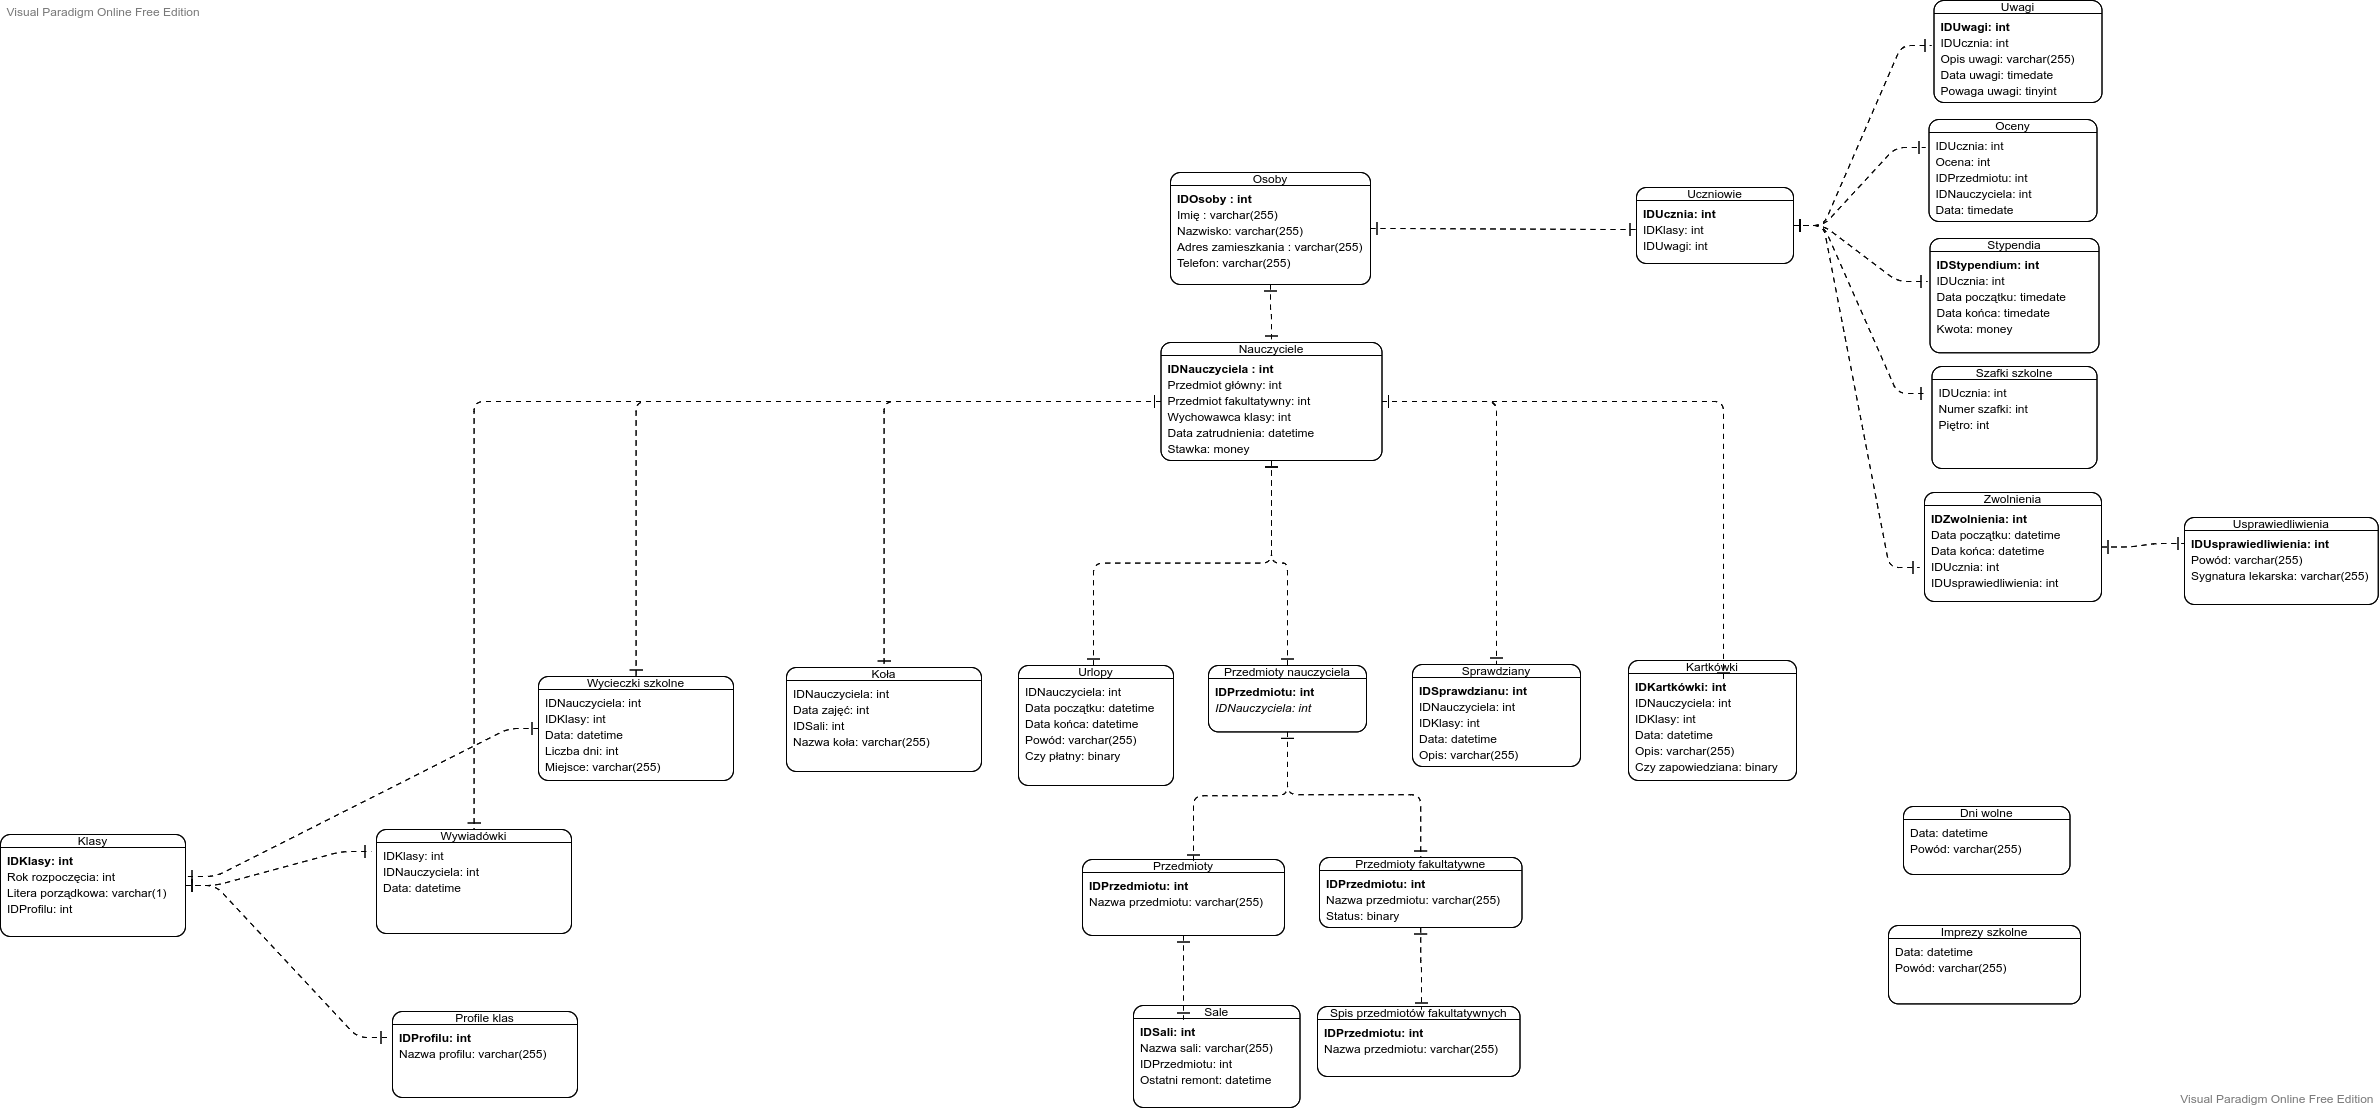
\includegraphics[width=\linewidth]{diagram_ER.png}
  \caption{Diagram ER}
  \label{Diagram ER}
\end{figure}

\newpage
\subsection{Diagram ER (SSMS)}

\begin{figure}[h]
  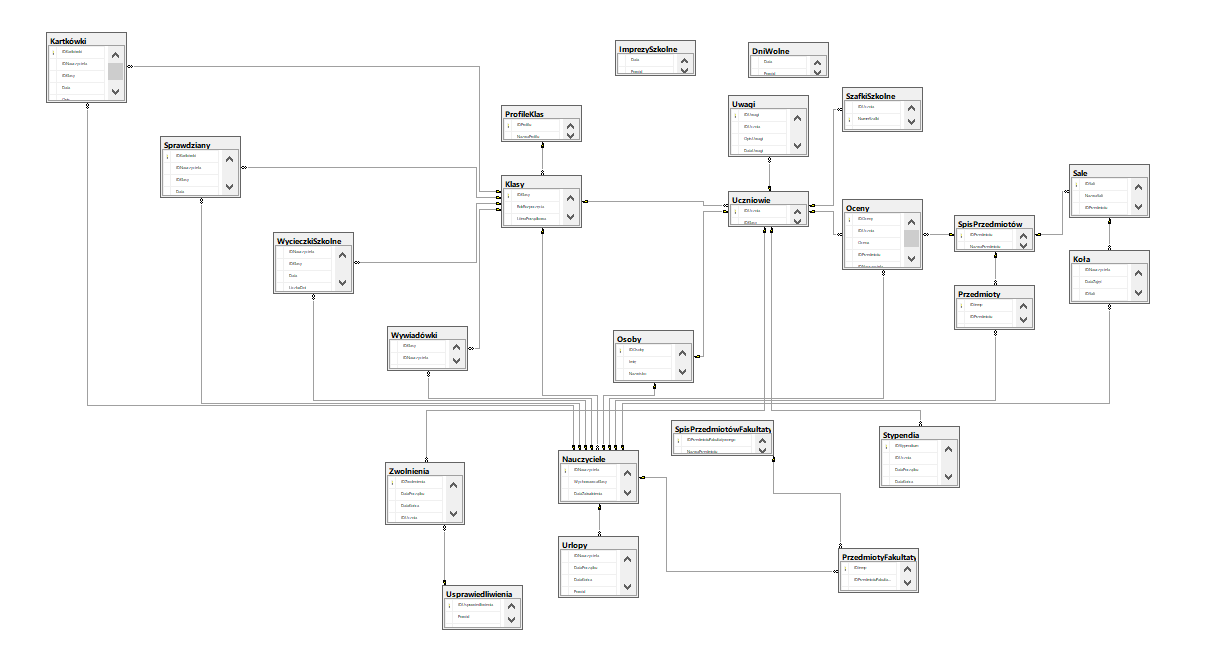
\includegraphics[width=\linewidth]{diagram_ER_SSMS.png}
  \caption{Diagram ER (SSMS)}
  \label{Diagram ER (SSMS)}
\end{figure}

\newpage
\section{Dokumentacja technicza}

\subsection{Tabele}

Wymagania projektu określały, że na każdą osobę pracującą przy projekcie wymagane jest zaimplementowanie 8 tabel, stąd też w tym rozdziale przedstawimy implementację 24 tabel.

\subsubsection{Osoby}
Jedna z podstawowych tabel bazy danych. Zawiera najistotniejsze dane o osobach uczestniczących do szkoły (nauczyciele i uczniowie) - ID, imię, nazwisko oraz telefon komórkowy.

\begin{minted}{sql}
CREATE TABLE Osoby
(
    IDOsoby INT IDENTITY(1,1) PRIMARY KEY,
    Imię VARCHAR(255) NOT NULL,
    Nazwisko VARCHAR(255) NOT NULL,
    Telefon VARCHAR(255)
)

INSERT INTO [Osoby](Imię, Nazwisko, Telefon) VALUES
('Wojciech', 'Węgrzyn', '+48 723 147 680'),
('Konrad', 'Nowak', NULL),
('Jakub', 'Łukasiewicz', NULL),
('John', 'Grady', '+01 134 423 423'),
('Adrian', 'Antkiewicz', '+48 534 322'),
('Michał', 'Gem', '+18 332 03 42'),
('Piotr', 'Niemiec', '+12 890 43 54'),
('Edward', 'Szczypka', '+12 345 54 23'),
('Jadwiga', 'Kowal', NULL),
('Iga', 'Świątek', NULL),
('Andrzej', 'Gołota', '+48 543 134 543')
\end{minted}

\subsubsection{Nauczyciele}
 Jedna z podstawowych tabel bazy danych. Zawiera informacje o tym jakiej klasy jest wychowawcą, kiedy został zatrudniony oraz ile zarabia miesięcznie.
 
 \begin{minted}{sql}
CREATE TABLE Nauczyciele
(
    IDNauczyciela INT REFERENCES Osoby(IDOsoby)
        ON UPDATE CASCADE ON DELETE CASCADE PRIMARY KEY,
    WychowawcaKlasy INT REFERENCES Klasy(IDKlasy),
    DataZatrudnienia DATETIME,
    Stawka MONEY,
)

INSERT INTO [Nauczyciele]
(IDNauczyciela, WychowawcaKlasy, DataZatrudnienia, Stawka)
VALUES
(4, NULL, GETDATE(), 5400),
(6, NULL, '20120802', 3000),
(7, NULL, '20011011', 15000),
(8, 1, '20130801', 2300),
(9, 2, '20200101', 4500)
\end{minted}
 
\newpage
 
\subsubsection{Uczniowie}
Tabela przyporządkowująca danemu uczniowi klasę, do której chodzi.
 
\begin{minted}{sql}
 --utworzenie tabeli
CREATE TABLE Uczniowie
(
    IDUcznia INT REFERENCES Osoby(IDOsoby) 
        ON UPDATE CASCADE ON DELETE CASCADE PRIMARY KEY,
    IDKlasy INT REFERENCES Klasy(IDKlasy) 
        ON UPDATE CASCADE ON DELETE CASCADE NOT NULL
)

--wstawienie uczniów
INSERT INTO [Uczniowie] (IDUcznia, IDKlasy) VALUES
(1, 1),
(2, 1),
(3, 1),
(5, 2),
(6, 2),
(10, 3),
(11, 3)
\end{minted}
 
 \subsubsection{Oceny}
Tabela zawierająca informację o ocenach, które dostał dany uczeń - jej wartość, jaki nauczyciel ją wystawił i z jakiego przedmiotu oraz data wystawienia jej.
 
\begin{minted}{sql}
--utworzenie tabeli
CREATE TABLE Oceny
(
    IDOceny INT IDENTITY(1,1) PRIMARY KEY NOT NULL,
    IDUcznia INT REFERENCES Uczniowie(IDUcznia),
    Ocena INT NOT NULL,
    IDPrzedmiotu INT REFERENCES SpisPrzedmiotów(IDPrzedmiotu)
        ON UPDATE CASCADE ON DELETE CASCADE NOT NULL,
    IDNauczyciela INT REFERENCES Nauczyciele(IDNauczyciela) NOT NULL,
    Data DATETIME
)

--wstawianie ocen
INSERT INTO [Oceny] (IDUcznia, Ocena, IDPrzedmiotu, IDNauczyciela, Data) VALUES
(1, 4, 1, 4, GETDATE()),
(1, 5, 1, 7, '20210216'),
(2, 2, 2, 7, '20210216'),
(3, 3, 2, 8, GETDATE()),
(10, 2, 3, 9, '20210105')
\end{minted}

\subsubsection{Przedmioty}
 Prosta tabela będąca łącznikiem między nauczycielem, a spisem przedmiotów. Zawiera tylko IDPrzedmiotu i IDNauczyciela.
 
 \begin{minted}{sql}
--utworzenie tabeli
CREATE TABLE Przedmioty
(
    IDtemp INT IDENTITY(1,1) PRIMARY KEY NOT NULL,
    IDPrzedmiotu INT REFERENCES SpisPrzedmiotów(IDPrzedmiotu) NOT NULL,
    IDNauczyciela INT REFERENCES Nauczyciele(IDNauczyciela)
        ON UPDATE CASCADE ON DELETE CASCADE NOT NULL
)

--wstawianie przedmiotów
INSERT INTO [Przedmioty](IDPrzedmiotu, IDNauczyciela) VALUES
(1,4),
(2,6),
(3,4),
(4,6),
(5,4),
(6,4)
\end{minted}

\subsubsection{Przedmioty fakultatywne}
 Prosta tabela będąca łącznikiem między nauczycielem a spisem przedmiotów. Zawiera tylko IDPrzedmiotu i IDNauczyciela.
 
 \begin{minted}{sql}
--utworzenie tabeli
CREATE TABLE PrzedmiotyFakultatywne
(
    IDtemp INT IDENTITY(1,1) PRIMARY KEY NOT NULL,
    IDPrzedmiotuFakultatywnego INT REFERENCES
        SpisPrzedmiotówFakultatywnych(IDPrzedmiotuFakultatywnego),
    IDNauczyciela INT REFERENCES Nauczyciele(IDNauczyciela)
        ON UPDATE CASCADE ON DELETE CASCADE NOT NULL
)

--wstawianie przedmiotów fakultatywnych
INSERT INTO [PrzedmiotyFakultatywne]
(IDPrzedmiotuFakultatywnego, IDNauczyciela) VALUES
(7,4),
(8,6)
\end{minted}

\subsubsection{Spis przedmiotów}
Prosta tabela przechowująca spis przedmiotów obowiązkowych z ich nazwami.

 \begin{minted}{sql}
--utworzenie tabeli
CREATE TABLE SpisPrzedmiotów
(
    IDPrzedmiotu INT PRIMARY KEY,
    NazwaPrzedmiotu VARCHAR(255)
)

--wstawianie przedmiotów
INSERT INTO [SpisPrzedmiotów](IDPrzedmiotu, NazwaPrzedmiotu) VALUES
(1, 'Matematyka'),
(2, 'Informatyka'),
(3, 'Chemia'),
(4, 'Język Polski'),
(5, 'Biologia'),
(6, 'Fizyka')
\end{minted}

\subsubsection{Spis przedmiotów fakultatywnych}
Prosta tabela przechowująca spis przedmiotów fakultatywnych z ich nazwami.

 \begin{minted}{sql}
--utworzenie tabeli
CREATE TABLE SpisPrzedmiotówFakultatywnych
(
    IDPrzedmiotuFakultatywnego INT PRIMARY KEY,
    NazwaPrzedmiotu VARCHAR(255)
)

--wstawianie przedmiotów fakultatywnych
INSERT INTO [SpisPrzedmiotówFakultatywnych]
(IDPrzedmiotuFakultatywnego, NazwaPrzedmiotu) VALUES
(7, 'Etyka'),
(8, 'Religia')
\end{minted}

 \subsubsection{Sprawdziany}
Tabela zawierająca informację o sprawdzianach przeprowadzanych w szkole. Przechowuje informacje o nauczycielu, który przeprowadza ten sprawdzian, klasę, która go pisała, datę pisania oraz krótki opis zawierający np. opis materiału, jaki obejmował dany sprawdzian.
 
\begin{minted}{sql}
--utworzenie tabeli
CREATE TABLE Sprawdziany
(
    IDSprawdzianu INT IDENTITY(1,1) PRIMARY KEY,
    IDNauczyciela INT REFERENCES Nauczyciele(IDNauczyciela)
        ON UPDATE CASCADE ON DELETE CASCADE NOT NULL,
    IDKlasy INT REFERENCES Klasy(IDKlasy)
        ON UPDATE CASCADE ON DELETE CASCADE NOT NULL,
    Data DATETIME,
    Opis VARCHAR(255)
)

--wstawianie sprawdzianu
INSERT INTO [Sprawdziany](IDNauczyciela, IDKlasy, Data, Opis) VALUES
(4, 1, '20211012', 'Rodziały 1-6'),
(8, 2, '20200110', 'Cały zakres materiału'),
(9, 2, '20211029', 'Rodziały 7-9')
\end{minted}

 \subsubsection{Kartkówki}
Tabela zwierająca informację o kartkówkach przeprowadzanych przez danego nauczyciela dla danej klasy wraz z datą, opisem oraz informacją, czy była ona zapowiedziana czy nie.
 
\begin{minted}{sql}
--utworzenie tabeli
CREATE TABLE Kartkówki
(
    IDKartkówki INT IDENTITY(1,1) PRIMARY KEY,
    IDNauczyciela INT REFERENCES Nauczyciele(IDNauczyciela)
        ON UPDATE CASCADE ON DELETE CASCADE NOT NULL,
    IDKlasy INT REFERENCES Klasy(IDKlasy)
        ON UPDATE CASCADE ON DELETE CASCADE NOT NULL,
    Data DATETIME,
    Opis VARCHAR(255),
    CzyZapowiedziana BIT
)

--wstawianie kartkówek
INSERT INTO [Kartkówki](IDNauczyciela, IDKlasy, Data, Opis, CzyZapowiedziana) VALUES
(4, 1, GETDATE(), 'Niezapowiedziana kartkówka z poprzedniej lekcji', 0),
(8, 2, '20200110', 'Poprzednie 3 tematy', 1)
\end{minted}

 \subsubsection{Uwagi}
Tabela poświęcona uwagom ucznia. Zawiera IDUcznia, który dostał uwagę, krótki opis, datę oraz skalę powagi otrzymanej uwagi (w skali od 1-3, gdzie im większa liczba, tym poważniejsza uwaga).
 
\begin{minted}{sql}
--utworzenie tabeli
CREATE TABLE Uwagi
(
    IDUwagi INT IDENTITY(1,1) PRIMARY KEY,
    IDUcznia INT REFERENCES Uczniowie(IDUcznia) 
        ON UPDATE CASCADE ON DELETE CASCADE NOT NULL,
    OpisUwagi VARCHAR(255),
    DataUwagi DATETIME,
    PowagaUwagi TINYINT NOT NULL
)

--dodawanie uwag
INSERT INTO [Uwagi](IDUcznia, OpisUwagi, DataUwagi, PowagaUwagi) VALUES
(1, 'Bujał się na krześle', GETDATE(), 1),
(1, 'Rozmawiał na lekcji', '20210302', 1),
(2, 'Ściągał na teście', GETDATE(), 2),
(3, 'Pobił kolegę', '20210411', 3)
\end{minted}

 \subsubsection{Stypendia}
Tabela poświęcona stypendium, które dostają najlepsi uczniowie. Zawiera IDUcznia, który je otrzymuje, datę rozpoczęcia i zakończenia wpłat oraz samą miesięczną kwotę stypendium.
 
\begin{minted}{sql}
--utworzenie tabeli
CREATE TABLE Stypendia
(
    IDStypendium INT IDENTITY(1,1) PRIMARY KEY,
    IDUcznia INT REFERENCES Uczniowie(IDUcznia) 
        ON UPDATE CASCADE ON DELETE CASCADE NOT NULL,
    DataPoczątku DATETIME,
    DataKońca DATETIME,
    Kwota MONEY
)

--przyznanie stypendium 
INSERT INTO [Stypendia](IDUcznia, DataPoczątku, DataKońca, Kwota) VALUES
(1, '20200901', '20210630', 500),
(2, '20190901', '20200630', 1000),
(5, '20190901', '20200630', 200)
\end{minted}

 \subsubsection{Sale}
Informacja zawierająca informację o salach znajdujących się w szkole. Każda sala ma swoją własną nazwę oraz przyporządkowany do niej jeden przedmiot. Dodatkowo zawiera również datę ostatniego remontu sali.
 
\begin{minted}{sql}
--utworzenie tabeli
CREATE TABLE Sale
(
    IDSali INT IDENTITY(1,1) PRIMARY KEY,
    NazwaSali VARCHAR(255),
    IDPrzedmiotu INT REFERENCES SpisPrzedmiotów(IDPrzedmiotu) 
        ON UPDATE CASCADE ON DELETE CASCADE,
    OstatniRemont DATETIME
)

--dodawanie sal
INSERT INTO [Sale](NazwaSali, IDPrzedmiotu, OstatniRemont) VALUES
('23A', 1, '19930304'),
('1A', 2, '18950213'),
('1B', 3, GETDATE()),
('2', NULL, '20101011'),
('Świetlica', NULL, '20100523')
\end{minted}

 \subsubsection{Klasy}
Tabela zawierająca klasy uczniów uczęszczających do szkoły. Tabela zawiera rok rozpoczęcia, literę porządkową (a, b itd.) oraz IDProfilu danej klasy.
 
\begin{minted}{sql}
--utworzenie tabeli
CREATE TABLE Klasy
(
    IDKlasy INT IDENTITY(1,1) PRIMARY KEY,
    RokRozpoczęcia INT NOT NULL,
    LiteraPorządkowa VARCHAR(1),
    IDProfilu INT REFERENCES ProfileKlas(IDProfilu) 
        ON UPDATE CASCADE ON DELETE CASCADE NOT NULL
)

--dodanie klasy
INSERT INTO [Klasy](RokRozpoczęcia, LiteraPorządkowa, IDProfilu) VALUES
(2019, 'A', 1),
(2019, 'B', 1),
(2018, 'A', 1),
(2018, 'B', 2),
(2017, NULL, 3)
\end{minted}

 \subsubsection{Profile klas}
Mała tabela zawierające IDProfilu oraz nazwę profilu klas w szkole.
 
\begin{minted}{sql}
--utworzenie tabeli
CREATE TABLE ProfileKlas
(
    IDProfilu INT IDENTITY(1,1) PRIMARY KEY,
    NazwaProfilu VARCHAR(255)
)

--dodanie profilów klas
INSERT INTO [ProfileKlas](NazwaProfilu) VALUES
('Mat-fiz'),
('Biol-chem'),
('Humanistyczny')
\end{minted}

 \subsubsection{Dni wolne}
Prosta tabela zawierająca datę oraz informację dotyczących dni wolnych podczas trwania roku szkolnego.
 
\begin{minted}{sql}
--utworzenie tabeli
CREATE TABLE DniWolne
(
    Data DATETIME,
    Powód VARCHAR(255)
)

--tworzenie dni wolnych
INSERT INTO [DniWolne](Data, Powód) VALUES
('20201111', 'Dzień Niepodległości'),
('20201223', 'Święta Bożego Narodzenia'),
('20201224', 'Święta Bożego Narodzenia'),
('20201225', 'Święta Bożego Narodzenia'),
('20201226', 'Święta Bożego Narodzenia'),
('20201231', 'Sylwester'),
('20210101', 'Nowy Rok')
\end{minted}

 \subsubsection{Wywiadówki}
Tabela przechowująca dane o wywiadówkach przeprowadzanych w trakcie roku szkolnego, zawierająca jaki nauczyciel dla jakiej klasy przeprowadzał daną wywiadówkę wraz z datą.
 
\begin{minted}{sql}
--utworzenie tabeli
CREATE TABLE Wywiadówki
(
	IDKlasy INT REFERENCES Klasy(IDKlasy) 
	    ON UPDATE CASCADE ON DELETE NOT NULL,
	IDNauczyciela INT REFERENCES Nauczyciele(IDNauczyciela) 
	    ON UPDATE CASCADE ON DELETE,
	Data DATETIME
)

--dodanie wywiadówki
INSERT INTO [Wywiadówki](IDKlasy, IDNauczyciela, DATA) VALUES
(1, 4, '20201012'),
(2, 8, '20201212'),
(3, 4, '20210120'),
(4, 9, '20210210')
\end{minted}

 \subsubsection{Koła}
Tabela przechowująca informacje odnośnie kół zainteresowań w szkole. Zawiera informacje o nauczycielu opiekującym się kołem, dacie odbywania się zajęć, salę, w której się odbywają spotkania oraz nazwę koła.
 
\begin{minted}{sql}
--utworzenie tabeli
CREATE TABLE Koła
(
	IDNauczyciela INT REFERENCES Nauczyciele(IDNauczyciela) 
	    ON UPDATE CASCADE ON DELETE NOT NULL,
	DataZajęć INT NOT NULL,
	IDSali INT REFERENCES Sale(IDSali) 
	    ON UPDATE CASCADE ON DELETE NOT NULL,
	NazwaKoła VARCHAR(255) NOT NULL
)

--wstawianie sal
INSERT INTO [Koła](IDNauczyciela, DataZajęć, IDSali, NazwaKoła) VALUES
(4, '20210210', 1, 'Koło Informatyczne'),
(4, '20210212', 1, 'Koło Matematyczne')
\end{minted}

 \subsubsection{Wycieczki szkolne}
 Tabela przechowująca informacje odnośnie wycieczek szkolnych, które odbyły się w trakcie trwania roku szkolnego. Każda wycieczka szkolna ma nauczyciela, który był podczas jej trwania opiekunem, klasę, jaka pojechała na tę wycieczkę, datę odbycia oraz czas trwania w dniach oraz miejsce, do którego się udali.
\begin{minted}{sql}
--utworzenie tabeli
CREATE TABLE WycieczkiSzkolne
(
    IDNauczyciela INT REFERENCES Nauczyciele(IDNauczyciela) 
        ON UPDATE CASCADE ON DELETE CASCADE NOT NULL,
    IDKlasy INT REFERENCES Klasy(IDKlasy) 
        ON UPDATE CASCADE ON DELETE CASCADE NOT NULL,
    Data DATETIME,
    LiczbaDni INT,
    Miejsce VARCHAR(255)
)

--wstawianie wycieczek
INSERT INTO [WycieczkiSzkolne](IDNauczyciela, IDKlasy, Data, LiczbaDni, Miejsce) VALUES
(4, 1, '20201010', 5, 'Zagrzeb'),
(4, 2, '20201201', 2, 'Kraków'),
(8, 1, '20210102', 1, 'Warszawa'),
(8, 3, '20201020', 4, 'Berlin'),
(9, 2, '20191012', 3, 'Lwów'),
(9, 1, '20191230', 1, 'Zakopane')
\end{minted}

 \subsubsection{Szafki szkolne}
 Prosta tabela przechowująca informację o szafce szkolnej danego ucznia, wraz z jej numerem oraz piętrem, na którym się znajduje.

\begin{minted}{sql}
--utworzenie tabeli
CREATE TABLE SzafkiSzkolne
(
    IDUcznia INT REFERENCES Uczniowie(IDUcznia) 
        ON UPDATE CASCADE ON DELETE CASCADE NOT NULL,
    NumerSzafki INT PRIMARY KEY,
    Piętro INT
)

--wstawienie szafki
INSERT INTO [SzafkiSzkolne](IDUcznia, NumerSzafki, Piętro) VALUES
(1, 10, 0),
(2, 11, 0),
(3, 12, 0),
(10, 33, 1),
(5, 1, 1),
(6, 2, 1),
(11, 3, 2)
\end{minted}

 \subsubsection{Imprezy szkolne}
Prosta tabela przechowująca informacja odnośnie imprez szkolnych, które odbyły się w trakcie roku wraz z datą oraz przyczyną zorganizowania.

\begin{minted}{sql}
--utworzenie tabeli
CREATE TABLE ImprezySzkolne
(
	Data DATETIME,
	Powód VARCHAR(255)
)

--wstawianie imprez
INSERT INTO [ImprezySzkolne](Data, Powód) VALUES
('20210102', 'Nowy Rok'),
('20200615', 'Zakończenie roku szkolnego'),
('20201010', 'Andrzejki'),
('20210214', 'Walentynki'),
(GETDATE(), 'Spontaniczna impreza')
\end{minted}

 \subsubsection{Urlopy}
Tabela zawierająca informacje odnośnie urlopów nauczycieli wraz z datami rozpoczęcia oraz zakończenia danego urlopy z podanym powodem oraz informacją, czy był płatny, czy nie.

\begin{minted}{sql}
--utworzenie tabeli
CREATE TABLE Urlopy
(
    IDNauczyciela INT REFERENCES Nauczyciele(IDNauczyciela) 
        ON UPDATE CASCADE ON DELETE CASCADE NOT NULL,
    DataPoczątku DATETIME NOT NULL,
    DataKońca DATETIME,
    Powód VARCHAR(255),
    CzyPłatny BIT NOT NULL,
)

--wstawianie urlopów
INSERT INTO [Urlopy](IDNauczyciela, DataPoczątku, DataKońca, Powód, CzyPłatny) VALUES
(4, '20210101', '20210102', 'Kac noworoczny', 0),
(4, '20210401', '20210430', 'Złamana noga', 1),
(8, '20201001', '20201230', 'Problemy rodzinne', 0)
\end{minted}

 \subsubsection{Zwolnienia}
Tabela przechowująca informacje odnośnie zwolnień ucznia wraz z datami początku i końca zwolnienia, z odnośnikiem do ucznia oraz usprawiedliwienia.

\begin{minted}{sql}
--utworzenie tabeli
CREATE TABLE Zwolnienia
(
    IDZwolenienia INT IDENTITY(1,1) PRIMARY KEY,
    DataPoczątku DATETIME,
    DataKońca DATETIME,
    IDUcznia INT REFERENCES Uczniowie(IDUcznia)
        ON UPDATE CASCADE ON DELETE CASCADE NOT NULL,
    IDUsprawiedliwienia INT REFERENCES Usprawiedliwienia(IDUsprawiedliwienia)
        ON UPDATE CASCADE ON DELETE CASCADE
)

--wstawianie zwolnień
INSERT INTO [Zwolnienia](DataPoczątku, DataKońca, IDUcznia, IDUsprawiedliwienia) VALUES
('20201010', '20201011', 1, NULL),
('20210302', '20210302', 2, 1)
\end{minted}

\subsubsection{Usprawiedliwienia}
Prosta table zawierająca informacje odnośnie usprawiedliwienia dla zwolnienia ucznia. Zawiera ona IDUsprawiedliwienia, powód oraz sygnaturę lekarską potwierdzającą to usprawiedliwienie.

\begin{minted}{sql}
--utworzenie tabeli
CREATE TABLE Usprawiedliwienia
(
    IDUsprawiedliwienia INT IDENTITY(1, 1) PRIMARY KEY,
    Powód VARCHAR(255),
    SygnaturaLekarska VARCHAR(255)
)

--wstawianie usprawiedliwienia 
INSERT INTO [Usprawiedliwienia](Powód, SygnaturaLekarska) VALUES
('Złamana noga', 'L/13/202'),
('Osłabienie', 'L/13/201'),
('Biegunka', 'L/01/01')
\end{minted}

\newpage

\section{Widoki oraz funkcje}

Wymogi zaliczenia projektu określają 10 poprawnie zaimplementowanych widoków oraz funkcji. Poniżej przedstawiamy pięć widoków oraz pięć funkcji.

\subsection{Widoki}

\subsubsection{Wyświetlanie nauczycieli}

Podany widok wyświetli listę nauczycieli z informacją na temat klas, które uczą. 

\begin{minted}{sql}
CREATE VIEW wyświetl_nauczycieli AS
SELECT A.Imię, A.Nazwisko, A.Telefon, C.RokRozpoczęcia, C.LiteraPorządkowa, D.NazwaProfilu
FROM Osoby A JOIN Nauczyciele B
ON A.IDOsoby = B.IDNauczyciela
JOIN Klasy C ON B.WychowawcaKlasy = C.IDKlasy
JOIN ProfileKlas D ON C.IDProfilu = D.IDProfilu
\end{minted}

Powyższy widok dla przykładowych danych zwraca następujące wartości:

\begin{figure}[h]
  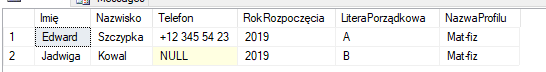
\includegraphics[width=\linewidth]{nauczyciele.png}
  \caption{Widok nauczycieli}
  \label{Widok nauczycieli}
\end{figure}

\subsubsection{Wyświetlanie sprawdzianów}

Widok ten wyświetli wszystkie sprawdziany wraz z ich datą, opisem oraz informacjami na temat nauczycieli oraz klas, których dotyczyły.

\begin{minted}{sql}
CREATE VIEW wyświetl_sprawdziany AS
SELECT A.Data, A.Opis, C.Imię AS [Imię Nauczyciela], 
C.Nazwisko AS [Nazwisko Nauczyciela], D.LiteraPorządkowa, D.RokRozpoczęcia, E.NazwaProfilu
FROM Sprawdziany A JOIN Nauczyciele B
ON A.IDnauczyciela = B.IDNauczyciela
JOIN Osoby C ON B.IDNauczyciela = C.IDOsoby
JOIN Klasy D ON A.IDKlasy = D.IDKlasy
JOIN ProfileKlas E ON D.IDProfilu = E.IDProfilu
ORDER BY E.NazwaProfilu
OFFSET 0 ROWS
\end{minted}

Powyższy widok dla przykładowych danych zwraca następujące wartości:

\begin{figure}[h]
  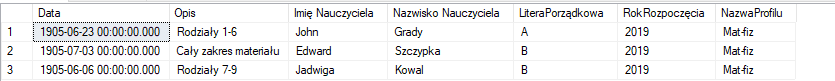
\includegraphics[width=\linewidth]{sprawdziany.png}
  \caption{Widok sprawdzianów}
  \label{Widok sprawdzianów}
\end{figure}

\subsubsection{Wyświetlanie uczniów}

Informacje na temat uczniów szkoły mogą zostać wyświetlone za pomocą poniższego widoku, zwracając informacje na temat ich danych osobowych, klasy do której uczęszczają oraz szafek, z których korzystają.

\begin{minted}{sql}
CREATE VIEW wyświetl_uczniów AS
SELECT A.Imię, A.Nazwisko, A.Telefon, 
C.RokRozpoczęcia, C.LiteraPorządkowa, 
D.NazwaProfilu, E.NumerSzafki, E.Piętro
FROM Osoby A JOIN Uczniowie B ON A.IDOsoby = B.IDUcznia
JOIN Klasy C ON B.IDKlasy = C.IDKlasy
JOIN ProfileKlas D ON C.IDProfilu = D.IDProfilu
JOIN SzafkiSzkolne E ON B.IDUcznia = E.IDUcznia
ORDER BY C.RokRozpoczęcia, D.NazwaProfilu, C.LiteraPorządkowa
OFFSET 0 ROWS
\end{minted}

Powyższy widok dla przykładowych danych zwraca następujące wartości:

\begin{figure}[h]
  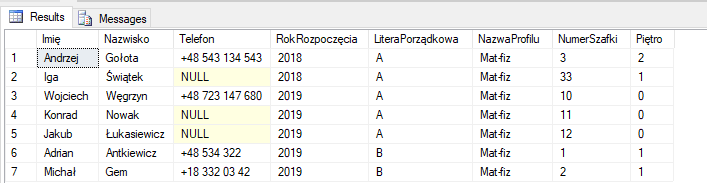
\includegraphics[width=\linewidth]{uczniowie.png}
  \caption{Widok uczniów}
  \label{Widok uczniów}
\end{figure}

\subsubsection{Trzy największe stypendia}

Widok wyświetlający trzy największe kwoty miesięczne ze wszystkich stypendiów w bazie, wyświetlając od największego do najmniejszego. 

\begin{minted}{sql}
GO
CREATE VIEW najwyzsze_stypendia
AS
SELECT TOP 3 S.Kwota FROM Stypendia S
ORDER BY S.Kwota DESC
GO

--wywołanie widoku
SELECT * FROM najwyzsze_stypendia
\end{minted}

\begin{figure}[h]
    \begin{center}
      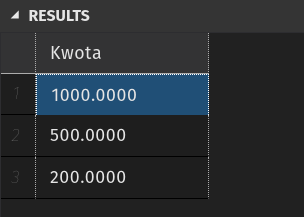
\includegraphics[width=0.5\linewidth]{najwyzsze_stypendia.png}
      \caption{Trzy największe stypendia w naszej testowej bazie}
      \label{Trzy największe stypendia w naszej testowej bazie}
    \end{center}
\end{figure}

\subsubsection{Ostatnio pisany sprawdzian}

Sprawdzenie szczegółów ostatnio dodanego do bazy sprawdziany można wykonać za pomocą następującego widoku:

\begin{minted}{sql}
GO
CREATE VIEW najnowszy_sprawdzian
AS
SELECT TOP 1 * FROM Sprawdziany AS S
ORDER BY S.Data DESC
GO

--użycie widoku
SELECT * FROM najnowszy_sprawdzian
\end{minted}

\begin{figure}[h]
    \begin{center}
      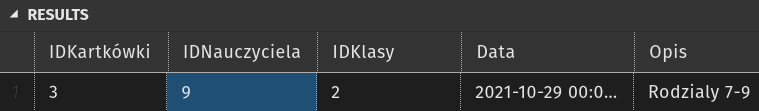
\includegraphics[width=\linewidth]{najnowszy_sprawdzian.png}
      \caption{Ostatnio dodany sprawdzian w testowej bazie.}
      \label{Ostatnio dodany sprawdzian w testowej bazie.}
    \end{center}
\end{figure}

\newpage
\subsection{Funkcje}

\subsubsection{Wypisanie uczniów danej klasy}

Funkcja pobierając ID danej klasy wypisuje wszystkich jej uczniów, wyświetlając ich imiona, nazwiska, numery telefonów oraz rok rozpoczęcia nauki. 

\begin{minted}{sql}
GO
CREATE FUNCTION dbo.wypisz_uczniow_danej_klasy (@ID AS INT)
RETURNS TABLE
AS
RETURN
SELECT O.Imię, O.Nazwisko, O.Telefon, K.RokRozpoczęcia
FROM Osoby O JOIN Uczniowie U
ON O.IDOsoby = U.IDUcznia
JOIN [Klasy] K
ON U.IDKlasy = K.IDKlasy
WHERE U.IDKlasy = @ID
GO
-- przykładowe wywołanie funkcji (wypisanie danych uczniów z klasy o ID == 1):
SELECT * FROM dbo.wypisz_uczniow_danej_klasy(1)
\end{minted}

Powyższa funkcja dla przykładowych danych i argumentu ID klasy = 1 zwraca następujące wartości:

\begin{figure}[h]
  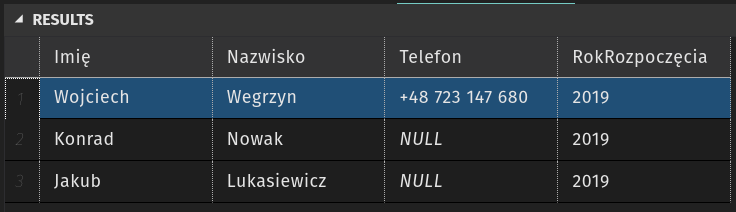
\includegraphics[width=\linewidth]{uczniowie_klasy.png}
  \caption{Uczniowie klasy o ID = 1}
  \label{Uczniowie klasy o ID = 1}
\end{figure}

\subsubsection{Wypisanie szczegółów ucznia}

Funkcja pobierając ID ucznia, wypisuje jego dane osobowe, szafkę szkolną oraz stypendium. 

\begin{minted}{sql}
GO
CREATE FUNCTION dbo.szczegoly_ucznia (@ID AS INT)
RETURNS TABLE
AS
RETURN
SELECT O.Imię, O.Nazwisko, O.Telefon, S.NumerSzafki, R.Kwota, R.DataPoczątku, R.DataKońca
FROM Osoby O JOIN Uczniowie U
ON O.IDOsoby = U.IDUcznia
FULL JOIN SzafkiSzkolne S
ON S.IDUcznia = U.IDUcznia
FULL JOIN Stypendia R
ON R.IDUcznia = U.IDUcznia
WHERE U.IDUcznia = @ID
GO
-- przykładowe wywołanie funkcji (wypisanie danych ucznia o ID = 5):
SELECT * FROM dbo.szczegoly_ucznia(5)
\end{minted}

Powyższa funkcja dla przykładowych danych i argumentu ID ucznia = 5 zwraca następujące wartości:

\begin{figure}[h]
  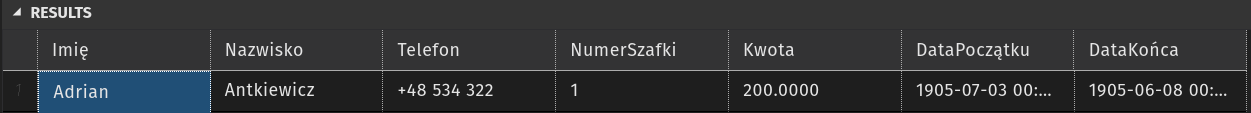
\includegraphics[width=\linewidth]{szczegoly_ucznia.png}
  \caption{Uczeń o ID = 5}
  \label{Uczeń o ID = 5}
\end{figure}

\subsubsection{Wyświetlanie kartkówek}

Funkcja ta jest bardzo podobna do widoku "Wyświetlanie sprawdzianów". Wyświetli wszystkie kartkówki wraz z ich datą, opisem oraz informacjami na temat nauczycieli oraz klas, których dotyczyły.

\begin{minted}{sql}
GO
CREATE FUNCTION wyświetl_kartkówki (@Stan AS BIT)
RETURNS TABLE
AS
RETURN
SELECT A.Data, A.Opis, C.Imię AS [Imię Nauczyciela], C.Nazwisko AS [Nazwisko Nauczyciela], D.LiteraPorządkowa, D.RokRozpoczęcia, E.NazwaProfilu
FROM Kartkówki A JOIN Nauczyciele B
ON A.IDnauczyciela = B.IDNauczyciela
JOIN Osoby C ON B.IDNauczyciela = C.IDOsoby
JOIN Klasy D ON A.IDKlasy = D.IDKlasy
JOIN ProfileKlas E ON D.IDProfilu = E.IDProfilu
WHERE A.CzyZapowiedziana = @Stan
GO

--przykładowe użycia
SELECT * FROM wyświetl_kartkówki(0)
SELECT * FROM wyświetl_kartkówki(1)
\end{minted}

Powyższe użycia dla przykładowych danych zwraca następujące wartości:

\begin{figure}[h]
  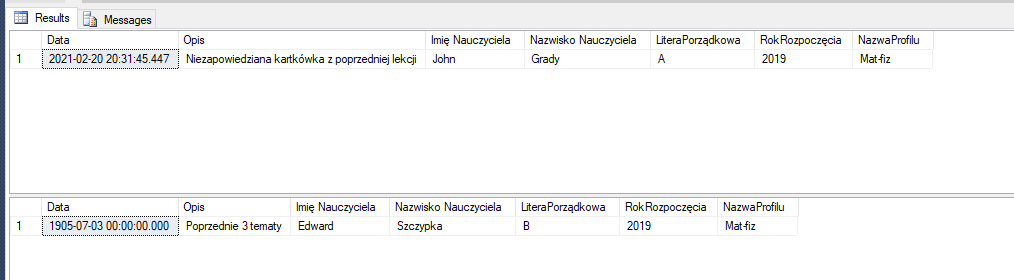
\includegraphics[width=\linewidth]{kartkowki.png}
  \caption{Widok kartkówek}
  \label{Widok kartkówek}
\end{figure}

\subsubsection{Wypisanie testów klasy}

Ponieważ nasza baza danych przechowuje osobno sprawdziany i kartkówki każdej z klasy zaistniała potrzeba implementacji funkcji, która wyświetli zarówno testy, jak i kartkówki dla klasy o podanym przez użytkownika ID. 

\begin{minted}{sql}
GO
CREATE FUNCTION dbo.testy_klasy (@ID AS INT)
RETURNS TABLE
AS
RETURN
(
    SELECT S.Data, S.Opis FROM Sprawdziany S
    WHERE @ID = S.IDKlasy
)
UNION ALL
(
    SELECT R.Data, R.Opis FROM Kartkówki R
    WHERE @ID = R.IDKlasy
)
GO
-- przykładowe wywołanie funkcji (wypisanie testów dla klasy o ID = 2):
SELECT * FROM dbo.testy_klasy(2)
\end{minted}

Powyższy wywołanie zwróci dla testowych danych następujący rezultat:

\begin{figure}[h]
  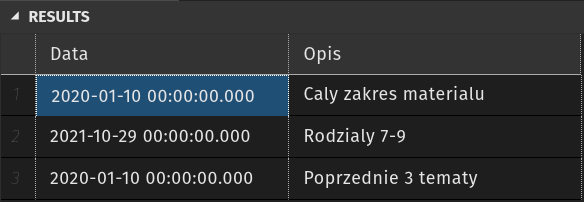
\includegraphics[width=\linewidth]{testy_klasy.png}
  \caption{Testy klasy o ID = 2}
  \label{Testy klasy o ID = 2}
\end{figure}

\subsubsection{Wypisanie nauczycieli o zarobkach większych niż podany parametr}

Ta funkcja za zadanie ma poinformować administrację o liczbie nauczycieli, których zarobki są powyżej określonej kwoty. 

\begin{minted}{sql}
CREATE FUNCTION dbo.liczba_nauczycieli_o_zarobkach
(@Zarobki MONEY)
RETURNS INT
AS BEGIN
RETURN (
    SELECT COUNT(N.IDNauczyciela)
    FROM Nauczyciele N
    WHERE N.Stawka >= @Zarobki
)
END
GO

--poniższe wywołanie dla przykładowych danych zwróci liczbę 3
SELECT dbo.liczba_nauczycieli_o_zarobkach(4000)
\end{minted}

\newpage

\section{Procedury i wyzwalacze}

Wymagania projektu: baza danych powinna być odpowiednio oprogramowana z wykorzystaniem procedur składowanych i wyzwalaczy (co najmniej po 5 procedur i po 5 wyzwalaczy).

\subsection{Wyzwalacze}

\subsubsection{Dodanie nauczyciela}

Operacja dodania nowego nauczyciela do bazy wywoła wyzwalacz, który określi czy operacja została wykonana pomyślnie oraz wskaże liczbę nauczycieli obecnie zapisanych do bazy danych.

\begin{minted}{sql}
GO
CREATE TRIGGER dodano_nauczyciela ON Nauczyciele
AFTER INSERT
AS BEGIN
DECLARE @msg NVARCHAR(55) = NULL
DECLARE @nr INT
SELECT @nr = COUNT(*) FROM Nauczyciele
SELECT 'Nauczyciel dodany pomyślnie.' [Stan operacji], 
CAST(@nr AS VARCHAR(10)) [Liczba nauczycieli w bazie]
END
GO

--przykładowe dodanie nauczyciela z wywołaniem triggera
INSERT INTO [Osoby](Imię, Nazwisko, Telefon) 
VALUES('Adam', 'Nowonauczycielski', '+48 132 147 444')
INSERT INTO [Nauczyciele](IDNauczyciela, WychowawcaKlasy, DataZatrudnienia, Stawka)
VALUES(12, 3, GETDATE(), 8000)
\end{minted}

Powyższa komenda wyświetli następujące informacje na naszych przykładowych danych:

\begin{figure}[h]
\begin{center}
  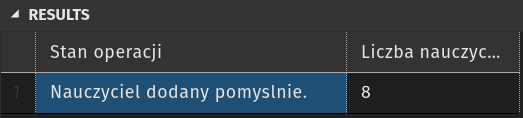
\includegraphics[width=0.6\linewidth]{dodanie_nauczyciela.png}
  \caption{Dodanie nauczyciela Adama Nowonauczycielskiego}
  \label{Dodanie nauczyciela Adama Nowonauczycielskiego}
\end{center}
\end{figure}

\subsubsection{Usunięcie ucznia}

Jeśli zdecydujemy się na usunięcie z naszej bazy danych ucznia, wywoła się wyzwalacz informujący o przebiegu operacji usunięcia ucznia oraz liczbie uczniów, którzy pozostali w bazie. 

\begin{minted}{sql}
GO
CREATE TRIGGER usunięcie_ucznia ON Uczniowie
AFTER DELETE
AS BEGIN
DECLARE @msg NVARCHAR(55) = NULL
DECLARE @nr INT
SELECT @nr = COUNT(*) FROM Uczniowie
SELECT 'Uczeń usunięty pomyślnie.' [Stan operacji], 
CAST(@nr AS VARCHAR(10)) [Liczba uczniów w bazie]
END
GO
--przykładowe usunięcie ucznia z wywołaniem triggera
DELETE FROM Uczniowie WHERE IDUcznia = 11
\end{minted}

Wykonanie powyższej operacji "DELETE" sprawi, że na naszym ekranie zostanie wyświetlony poniższy komunikat:

\begin{figure}[h]
\begin{center}
  \includegraphics[width=0.6\linewidth]{usunięcie_ucznia.png}
  \caption{Usunięcie ucznia o jego ID równym 11}
  \label{Usunięcie ucznia o jego ID równym 11}
\end{center}
\end{figure}

\subsubsection{Sprawdzenie liczby klas}

Koncept naszej bazy danych zakłada, że nie może istnieć klasa bez uczniów. Stąd też powstała potrzeba implementacji wyzwalacza, który uniemożliwi dodanie nowej klasy do naszej bazy danych w przypadku, gdyby było zbyt mało uczniów, aby stworzyć nową klasę. Nasz wyzwalacz sprawdza liczbę uczniów w całej szkole i nie zezwala na sytuację dodania klasy, do której nie można byłoby przypisać uczniów. Nasz wyzwalacz nie sprawdza, czy nie występuje na przykład sytuacja, że do naszej nowej klasy można byłoby dodać tylko jednego ucznia - akceptujemy taką sytuację, zakładając że wtedy możemy do nowej klasy przepisać uczniów z klas, które obecnie już w bazie danych się znajdują. 

\begin{minted}{sql}
CREATE TRIGGER sprawdzenie_liczy_klas ON Klasy
AFTER INSERT
AS
IF (SELECT COUNT(IDKlasy) FROM Klasy) > (SELECT COUNT(IDUcznia) FROM Uczniowie)
ROLLBACK
RAISERROR('Nie można dodać klasy, ponieważ jest za mało uczniów.', 16, 1)
GO
--przykładowe dodanie klasy z wywołaniem triggera
INSERT INTO [Klasy](RokRozpoczęcia, LiteraPorządkowa, IDProfilu) VALUES
(2012, 'A', 1),
(2012, 'B', 1),
(2012, 'C', 2),
(2012, 'D', 2),
(2012, 'E', 3),
(2012, 'F', 3)
\end{minted}

Powyższe dodanie szeregu klas spowoduje wycofanie transakcji oraz wyświetlenie następującego błędu, informującego o powodzie odrzucenia transakcji:

\begin{figure}[h]
\begin{center}
  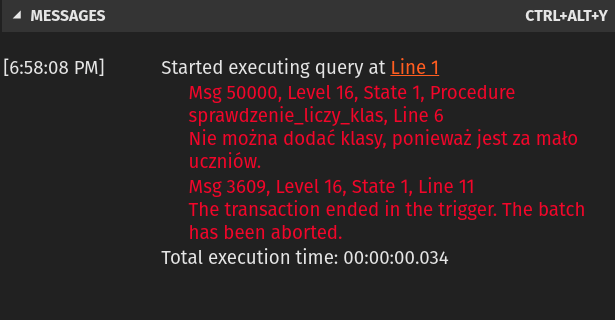
\includegraphics[width=0.6\linewidth]{sprawdzenie_liczby_klas.png}
  \caption{Błąd, wyświetlający się jeśli dodamy więcej klas niż uczniów.}
  \label{Błąd, wyświetlający się jeśli dodamy więcej klas niż uczniów.}
 \end{center}
\end{figure}

\subsubsection{Sprawdzenie możliwości zorganizowania imprezy szkolnej}

Nasza baza danych posiada zaimplementowane sprawdzenie możliwości dodania nowej imprezy szkolnej. Z racji, że uczniowie powinni się uczyć, a nie obijać, sprawdzamy czy data nowo dodanej imprezy szkolnej została ustalona na dzień wolny od nauki. Jeśli nie, to transakcja zostaje wycofana.

\begin{minted}{sql}
CREATE TRIGGER impreza_wolne ON ImprezySzkolne
AFTER INSERT
AS 
DECLARE
@Data INT
BEGIN
IF NOT EXISTS (
    SELECT Data FROM DniWolne d
    WHERE d.Data = @Data
    )
ROLLBACK
RAISERROR('Nie można zorganizować imprezy w dzień nauki.', 16, 1)
END

--dodanie przykładowej imprezy
INSERT INTO [ImprezySzkolne](Data, Powód) VALUES
(2021-03-30, 'Bo nie chce się nam uczyć')
\end{minted}

Powyższy "INSERT" wywoła następujący błąd:

\begin{figure}[h]
\begin{center}
  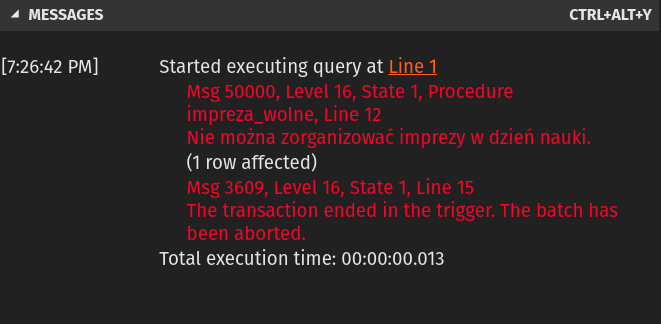
\includegraphics[width=0.75\linewidth]{impreza_wolne.png}
  \caption{Błąd, wyświetlający się jeśli dodamy impreze w dzień nauki.}
  \label{Błąd, wyświetlający się jeśli dodamy impreze w dzień nauki.}
\end{center}
\end{figure}

\subsubsection{Średnia ocen uczniów po dodaniu oceny}

Ze względu na rzadkie wstawianie nowych ocen do naszej bazy danych możemy pozwolić sobie na implementację wyzwalacza, który po każdej nowo dodanej ocenie będzie wyliczał średnią wszystkich ocen wszystkich uczniów.

\begin{minted}{sql}
CREATE TRIGGER srednia_ocen ON Oceny
AFTER INSERT
AS
BEGIN
    SELECT AVG(O.Ocena) AS [Srednia], O.IDUcznia 
    FROM Oceny AS O
    GROUP BY O.IDUcznia
END

--przykładowe dodanie oceny, zmieniające średnią
INSERT INTO [Oceny]
(IDUcznia, Ocena, IDPrzedmiotu, IDNauczyciela, Data)
VALUES
(1, 1, 2, 4, GETDATE())
\end{minted}

\begin{figure}[h]
\begin{center}
  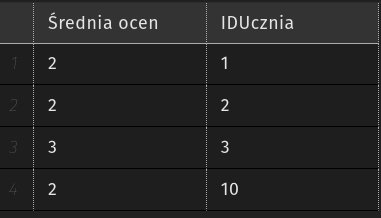
\includegraphics[width=0.5\linewidth]{srednia_ocen.png}
  \caption{Niestety, uczniowie naszej testowej bazy danych nie mogą pochwalić się zbyt dobrymi osiągnięciami w nauce...}
  \label{Niestety, uczniowie naszej testowej bazy danych nie mogą pochwalić się zbyt dobrymi osiągnięciami w nauce...}
  \end{center}
\end{figure}

\subsection{Procedury}

\subsubsection{Dodanie przedmiotu do bazy}

\begin{minted}{sql}
ALTER PROCEDURE dodaj_przedmiot
@nazwa VARCHAR(255)
AS
BEGIN
DECLARE @count INT
SET @count = (SELECT COUNT(*) FROM SpisPrzedmiotów)
SET @count = @count + 1;
IF NOT EXISTS (SELECT * FROM SpisPrzedmiotów WHERE NazwaPrzedmiotu=@nazwa)
INSERT INTO [SpisPrzedmiotów](IDPrzedmiotu, NazwaPrzedmiotu) VALUES (@count, @nazwa)
ELSE 
PRINT 'Taki przedmiot już istnieje'
END
\end{minted}

\subsubsection{Liczba uczniów w szkole}

\begin{minted}{sql}
CREATE PROCEDURE ile_uczniów
AS
BEGIN
SELECT COUNT(*) FROM Uczniowie
END
\end{minted}

\subsubsection{Sprawdzenie, czy podana osoba istnieje}

\begin{minted}{sql}
CREATE PROCEDURE czy_istnieje_osoba
@imie VARCHAR(255),
@nazwisko VARCHAR(255)
AS
BEGIN
IF EXISTS (SELECT * FROM Osoby WHERE Imię=@imie AND Nazwisko=@nazwisko)
PRINT 'TAK'
ELSE
PRINT 'NIE'
END
\end{minted}

\subsubsection{Określenie liczby wywiadówek w klasie}

\begin{minted}{sql}
CREATE PROCEDURE ile_wywiadówek
@klasa INT
AS
BEGIN
DECLARE @count INT
SET @count = (SELECT COUNT(*) FROM Wywiadówki WHERE IDKlasy=@klasa)
PRINT @count
END
\end{minted}

\subsubsection{Dodanie uwagi dla ucznia}

\begin{minted}{sql}
ALTER PROCEDURE dodaj_uwagę
@imię VARCHAR(255),
@nazwisko VARCHAR(255),
@uwaga VARCHAR(255),
@powaga_uwagi INT
AS
BEGIN
DECLARE @ID INT
IF EXISTS (SELECT IDOsoby FROM Osoby WHERE Imię=@imię AND Nazwisko=@nazwisko)
BEGIN
SET @ID = (SELECT IDOsoby FROM Osoby WHERE Imię=@imię AND Nazwisko=@nazwisko);
INSERT INTO [Uwagi](IDUcznia, OpisUwagi, DataUwagi, PowagaUwagi) 
VALUES (@ID, @uwaga, GETDATE(), @powaga_uwagi)
END
ELSE
PRINT 'Taki uczeń nie istnieje'
END
\end{minted}

\end{document}